\clearpage







\begin{figure}[hbt!]
	\caption{Leftmost Stock Price Digit and Probability of Sale, \\ Prices Increasing Sample \\ Limit Order Robustness Tests}%
	\label{fig:left_digit_sell_decrease_sellsample}%
	\centering%	
	\bigskip
	\subfigure[Excluding Pre-Market and After-Hours Sells (Outside 8am to 4:30pm)]{	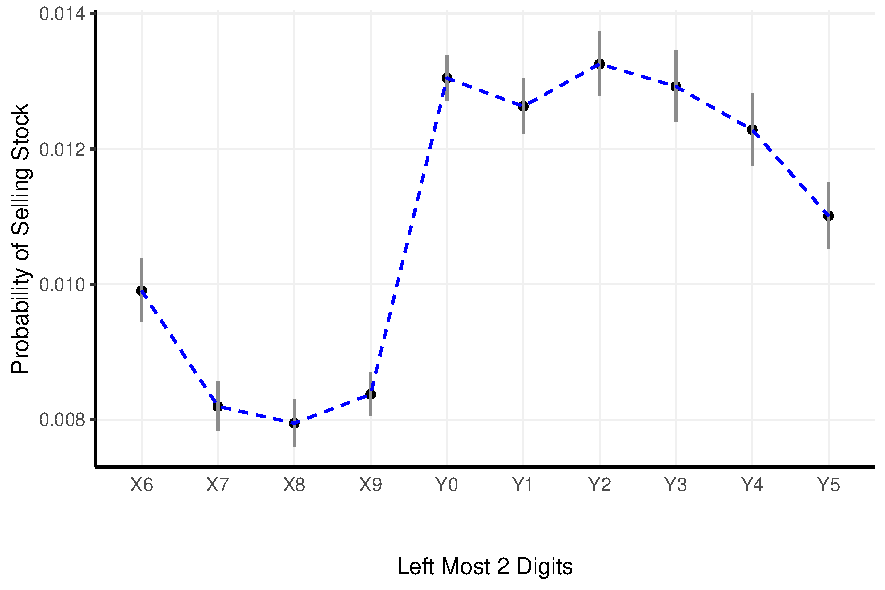
\includegraphics[width=0.45\textwidth]{figures/outside_hoursLeft2increase_probCI_quarter.pdf}
		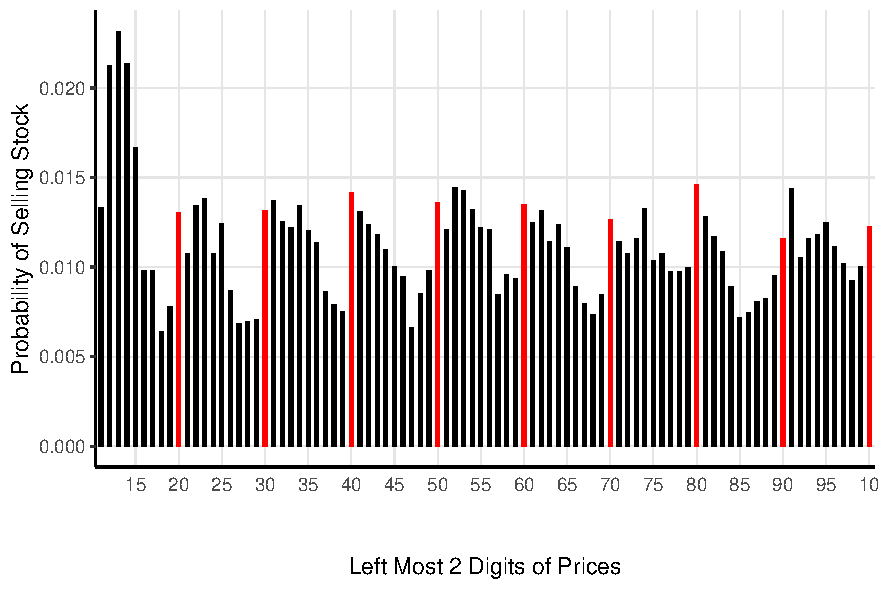
\includegraphics[width=0.45\textwidth]{figures/outside_hours2left_increase_quarter.pdf}	
	}
	\subfigure[Excluding Sells with Login the Day Before or Weekend Logins for Monday Sells]{
		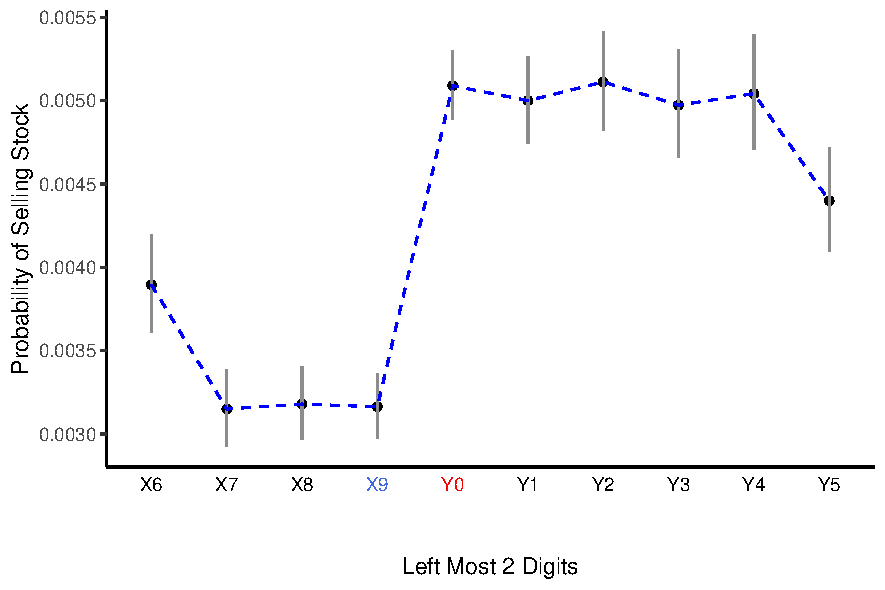
\includegraphics[width=0.45\textwidth]{figures/no_yest_loginLeft2increase_probCI_quarter.pdf}
		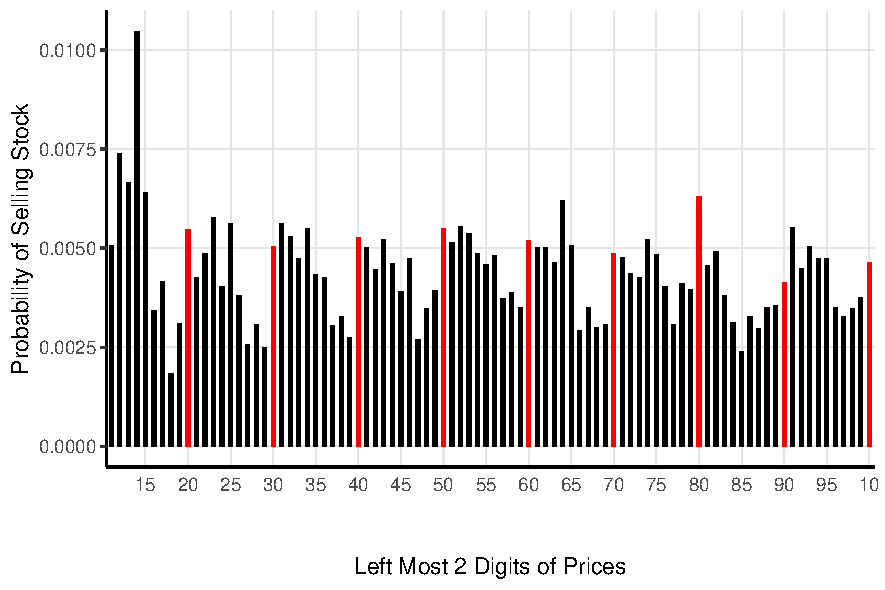
\includegraphics[width=0.45\textwidth]{figures/no_yest_login2left_increase_quarter.pdf}
	}
	\subfigure[Including Only FTSE100 Stocks]{
		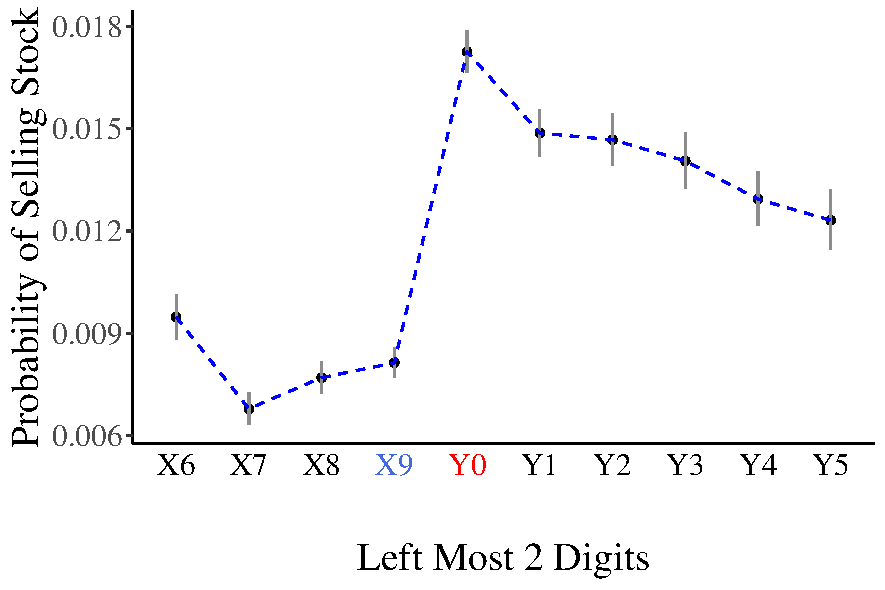
\includegraphics[width=0.45\textwidth]{figures/liquidLeft2increase_probCI_quarter.pdf}
		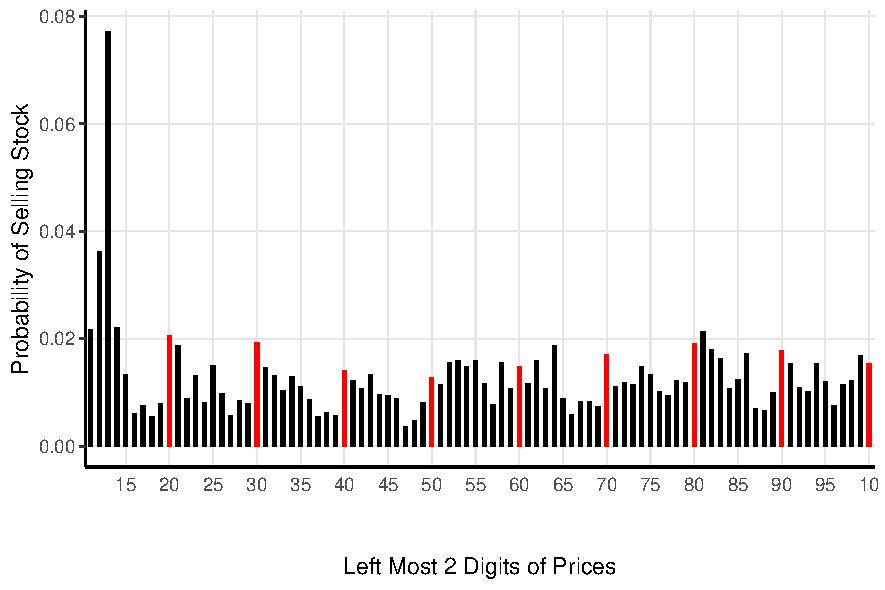
\includegraphics[width=0.45\textwidth]{figures/liquid2left_increase_quarter.pdf}		}
		\subfigure[Excluding Accounts with Potential Limit Orders (Linnainmaa, 2010)]{
		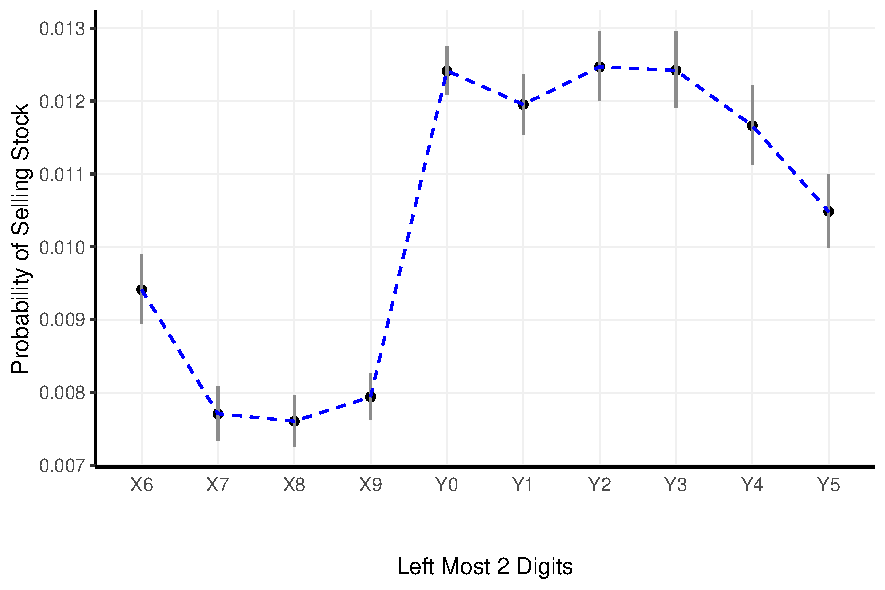
\includegraphics[width=0.45\textwidth]{figures/potential_lmLeft2increase_probCI_quarter.pdf}
		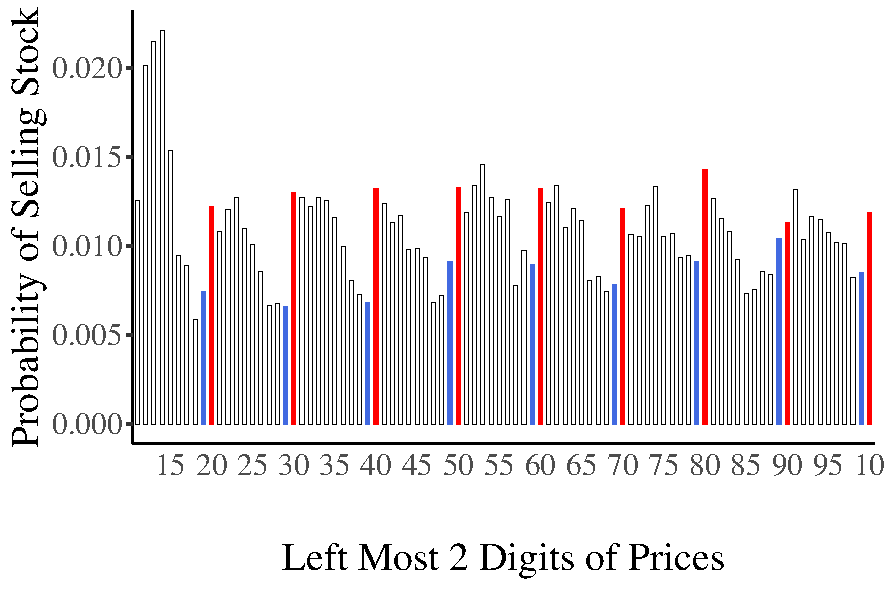
\includegraphics[width=0.45\textwidth]{figures/potential_lm2left_increase_quarter.pdf}
	}
	\fignote{£$Y$ in the X-axes is equivalent to £$X+1$ (e.g., £X9 could include £0.19, £1.9, £19, etc., while £Y0 could include £0.20, £2.0, £20, etc.). Panels A, B and C show equal size bins of 1p, 10p and £1, respectively. Panel A drops 0.018\% of sells, Panel B drops 61\% of sells, Panel C drops 76\% of sells, and Panel D drops 11\% of sells.} 

\end{figure}
\clearpage


\begin{table}[ht]\footnotesize
	\caption{Price Increasing Sample \\ Limit Order Robustness Tests}
	\label{tab:reg_subsamples_increase}
	\bigskip
	
	\begin{adjustbox}{center}
		\estauto{l c c c c c c  }<\multicolumn{6}{c}{Panel (A): Excluding Pre-Market and After-Hours Sells (Outside 8am to 4:30pm)} \\>{
			& \multicolumn{5}{c}{$Probability\:  of\:  Sale_{ijt}=1$} \\ 
			%	\cmidrule(rr){2-7}
			& \multicolumn{1}{c}{(1)} & \multicolumn{1}{c}{(2)} & \multicolumn{1}{c}{(3)} & \multicolumn{1}{c}{(4)} & 
			\multicolumn{1}{c}{(5)} & \\ 
			\midrule
			\\[-2.1ex] Above Y0 = 1 (in Range Y0 to Y5) & 0.0042{***} & 0.0053{***} & 0.0048{***} & 0.0052{***} & 0.0059{***} \\ 
  & (0.0001) & (0.0002) & (0.0002) & (0.0002) & (0.0002) \\ 
  Stock Digits Y0 to Y5 &  & -0.0003{***} & -0.0004{***} & -0.0005{***} & -0.0007{***} \\ 
  &  & (0.0000) & (0.0000) & (0.0000) & (0.0000) \\ 
  Stock Digits X6 to X9 &  & -0.0005{***} & -0.0003{***} & -0.0002{***} & -0.0002{***} \\ 
  &  & (0.0001) & (0.0001) & (0.0001) & (0.0001) \\ 
  Constant & 0.0084{***} & 0.0078{***} & 0.0064{***} &  &  \\ 
  & (0.0001) & (0.0001) & (0.0007) &  &  \\ 
 Day FE & NO & NO & YES & YES & YES \\ 
Industry FE & NO & NO & YES & YES & YES \\ 
Account FE & NO & NO & NO & YES & YES \\ 
Stock FE & NO & NO & NO & NO & YES \\ 
Observations & \multicolumn{1}{c}{4,993,803} & \multicolumn{1}{c}{4,993,803} & \multicolumn{1}{c}{4,993,803} & \multicolumn{1}{c}{4,993,803} & \multicolumn{1}{c}{4,993,803} \\ 
R$^{2}$ & \multicolumn{1}{c}{0.0004} & \multicolumn{1}{c}{0.0004} & \multicolumn{1}{c}{0.0018} & \multicolumn{1}{c}{0.0683} & \multicolumn{1}{c}{0.0730} \\ 
 
		}
	\end{adjustbox}
	
	\bigskip
	
	\begin{adjustbox}{center}
		\estauto{l c c c c c c  }<\multicolumn{6}{c}{Panel (B): Excluding Sells with Login the Day Before or Weekend Logins for Monday Sells} \\>{
			& \multicolumn{5}{c}{$Probability\:  of\:  Sale_{ijt}=1$} \\ 
			%	\cmidrule(rr){2-7}
			& \multicolumn{1}{c}{(1)} & \multicolumn{1}{c}{(2)} & \multicolumn{1}{c}{(3)} & \multicolumn{1}{c}{(4)} & 
			\multicolumn{1}{c}{(5)} & \\ 
			\midrule
			\\[-2.1ex] Above Y0 = 1 (in Y0 - Y5) & 0.0016{***} & 0.0021{***} & 0.0020{***} & 0.0023{***} & 0.0025{***} \\ 
  & (0.0001) & (0.0001) & (0.0001) & (0.0001) & (0.0001) \\ 
  Digits Y0 - Y5 &  & -0.0001{***} & -0.0001{***} & -0.0002{***} & -0.0003{***} \\ 
  &  & (0.0000) & (0.0000) & (0.0000) & (0.0000) \\ 
  Digits X6 - X9 &  & -0.0002{***} & -0.0002{***} & -0.0002{***} & -0.0002{***} \\ 
  &  & (0.0000) & (0.0000) & (0.0000) & (0.0000) \\ 
  Constant & 0.0031{***} & 0.0028{***} & 0.0012{***} &  &  \\ 
  & (0.0001) & (0.0001) & (0.0003) &  &  \\ 
 Day FE & NO & NO & YES & YES & YES \\ 
Industry FE & NO & NO & YES & YES & YES \\ 
Account FE & NO & NO & NO & YES & YES \\ 
Stock FE & NO & NO & NO & NO & YES \\ 
Observations & \multicolumn{1}{c}{4,834,411} & \multicolumn{1}{c}{4,834,411} & \multicolumn{1}{c}{4,834,411} & \multicolumn{1}{c}{4,834,411} & \multicolumn{1}{c}{4,834,411} \\ 
R$^{2}$ & \multicolumn{1}{c}{0.0002} & \multicolumn{1}{c}{0.0002} & \multicolumn{1}{c}{0.0010} & \multicolumn{1}{c}{0.0616} & \multicolumn{1}{c}{0.0643} \\ 
 
		}
	\end{adjustbox}
	\fignote{Panels A, B and C show equal size bins of 1p, 10p and £1, respectively. Panel A drops 0.018\% of sells, Panel B drops 61\% of sells, Panel C drops 76\% of sells, and Panel D drops 11\% of sells.}
\end{table}



\begin{table}[ht]\footnotesize
	\caption{Price Increasing Sample \\ Limit Order Robustness Tests}
	\label{tab:reg_subsamples_increase}
	\bigskip
	
	\begin{adjustbox}{center}
		\estauto{l c c c c c c  }<\multicolumn{6}{c}{Panel (C): Including Only FTSE100 Stocks} \\>{
			& \multicolumn{5}{c}{$Probability\:  of\:  Sale_{ijt}=1$} \\ 
			%	\cmidrule(rr){2-7}
			& \multicolumn{1}{c}{(1)} & \multicolumn{1}{c}{(2)} & \multicolumn{1}{c}{(3)} & \multicolumn{1}{c}{(4)} & 
			\multicolumn{1}{c}{(5)} & \\ 
			\midrule
			\\[-2.1ex] Above Y0 = 1 (in Range Y0 to Y5) & 0.0070{***} & 0.0090{***} & 0.0087{***} & 0.0096{***} & 0.0098{***} \\ 
  & (0.0002) & (0.0003) & (0.0003) & (0.0004) & (0.0004) \\ 
  Stock Digits Y0 to Y5 &  & -0.0010{***} & -0.0009{***} & -0.0009{***} & -0.0009{***} \\ 
  &  & (0.0001) & (0.0001) & (0.0001) & (0.0001) \\ 
  Stock Digits X6 to X9 &  & -0.0001 & -0.0001 & -0.0005{***} & -0.0005{***} \\ 
  &  & (0.0001) & (0.0001) & (0.0001) & (0.0001) \\ 
  Constant & 0.0079{***} & 0.0077{***} & 0.0259{***} &  &  \\ 
  & (0.0002) & (0.0002) & (0.0013) &  &  \\ 
 Day FE & NO & NO & YES & YES & YES \\ 
Industry FE & NO & NO & YES & YES & YES \\ 
Account FE & NO & NO & NO & YES & YES \\ 
Stock FE & NO & NO & NO & NO & YES \\ 
Observations & \multicolumn{1}{c}{1,126,143} & \multicolumn{1}{c}{1,126,143} & \multicolumn{1}{c}{1,126,143} & \multicolumn{1}{c}{1,126,143} & \multicolumn{1}{c}{1,126,143} \\ 
R$^{2}$ & \multicolumn{1}{c}{0.0010} & \multicolumn{1}{c}{0.0012} & \multicolumn{1}{c}{0.0025} & \multicolumn{1}{c}{0.1024} & \multicolumn{1}{c}{0.1031} \\ 
 
		}
	\end{adjustbox}
	
\begin{adjustbox}{center}
	\estauto{l c c c c c c  }<\multicolumn{6}{c}{Panel (D): Excluding Accounts with Potential Limit Orders (Linnainmaa, 2010)} \\>{
		& \multicolumn{5}{c}{$Probability\:  of\:  Sale_{ijt}=1$} \\ 
		%	\cmidrule(rr){2-7}
		& \multicolumn{1}{c}{(1)} & \multicolumn{1}{c}{(2)} & \multicolumn{1}{c}{(3)} & \multicolumn{1}{c}{(4)} & 
		\multicolumn{1}{c}{(5)} & \\ 
		\midrule
		\\[-2.1ex] Above Y0 = 1 (in Range Y0 to Y5) & 0.0041{***} & 0.0052{***} & 0.0048{***} & 0.0052{***} & 0.0058{***} \\ 
  & (0.0001) & (0.0002) & (0.0002) & (0.0002) & (0.0002) \\ 
  Stock Digits Y0 to Y5 &  & -0.0003{***} & -0.0004{***} & -0.0005{***} & -0.0007{***} \\ 
  &  & (0.0000) & (0.0000) & (0.0000) & (0.0000) \\ 
  Stock Digits X6 to X9 &  & -0.0004{***} & -0.0003{***} & -0.0003{***} & -0.0002{***} \\ 
  &  & (0.0001) & (0.0001) & (0.0001) & (0.0001) \\ 
  Constant & 0.0081{***} & 0.0075{***} & 0.0060{***} &  &  \\ 
  & (0.0001) & (0.0001) & (0.0007) &  &  \\ 
 Day FE & NO & NO & YES & YES & YES \\ 
Industry FE & NO & NO & YES & YES & YES \\ 
Account FE & NO & NO & NO & YES & YES \\ 
Stock FE & NO & NO & NO & NO & YES \\ 
Observations & \multicolumn{1}{c}{4,671,200} & \multicolumn{1}{c}{4,671,200} & \multicolumn{1}{c}{4,671,200} & \multicolumn{1}{c}{4,671,200} & \multicolumn{1}{c}{4,671,200} \\ 
R$^{2}$ & \multicolumn{1}{c}{0.0004} & \multicolumn{1}{c}{0.0004} & \multicolumn{1}{c}{0.0016} & \multicolumn{1}{c}{0.0695} & \multicolumn{1}{c}{0.0740} \\ 
 
	}
\end{adjustbox}
	\fignote{Panels A, B and C show equal size bins of 1p, 10p and £1, respectively. Panel A drops 0.018\% of sells, Panel B drops 61\% of sells, Panel C drops 76\% of sells, and Panel D drops 11\% of sells.}
\end{table}
\clearpage

\begin{figure}[hbt!]
	\caption{Leftmost Stock Price Digit and Probability of Sale, Quarterly Sample}%
	\label{fig:left_digit_sell_main}%
	\centering%	
	\bigskip
	\subfigure[Price Increasing]{
		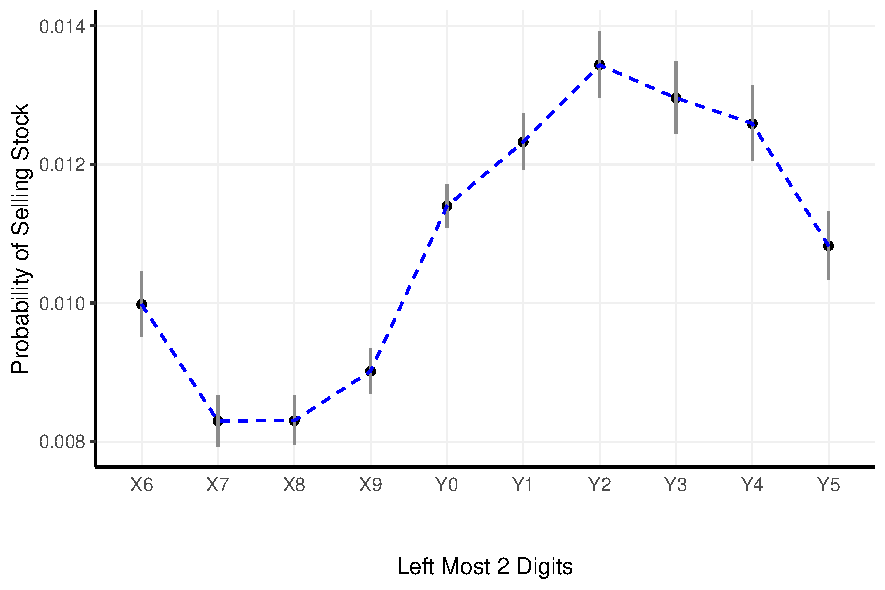
\includegraphics[width=0.45\textwidth]{figures/Left2increase_probCI_quarter.pdf}
		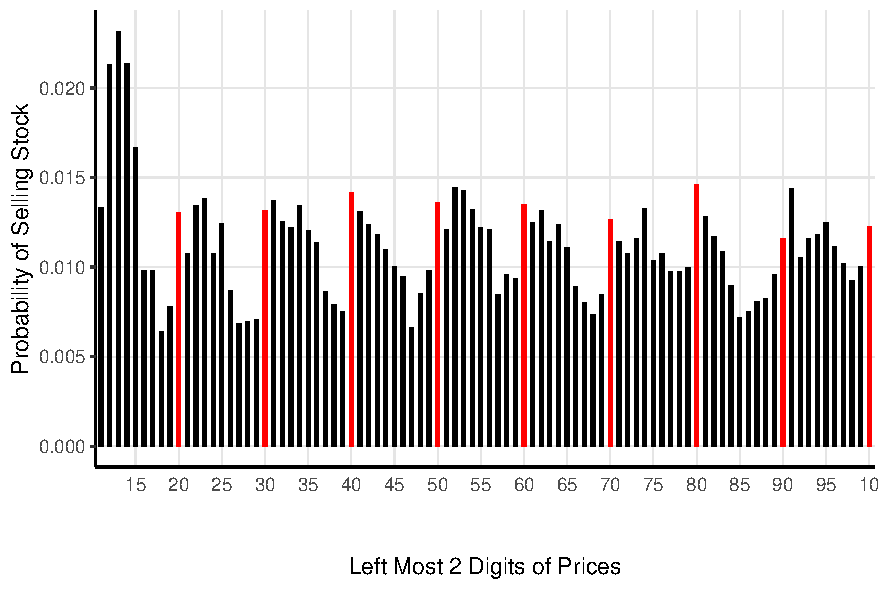
\includegraphics[width=0.45\textwidth]{figures/2left_increase_quarter.pdf}	
	}
	\subfigure[Price Decreasing]{
		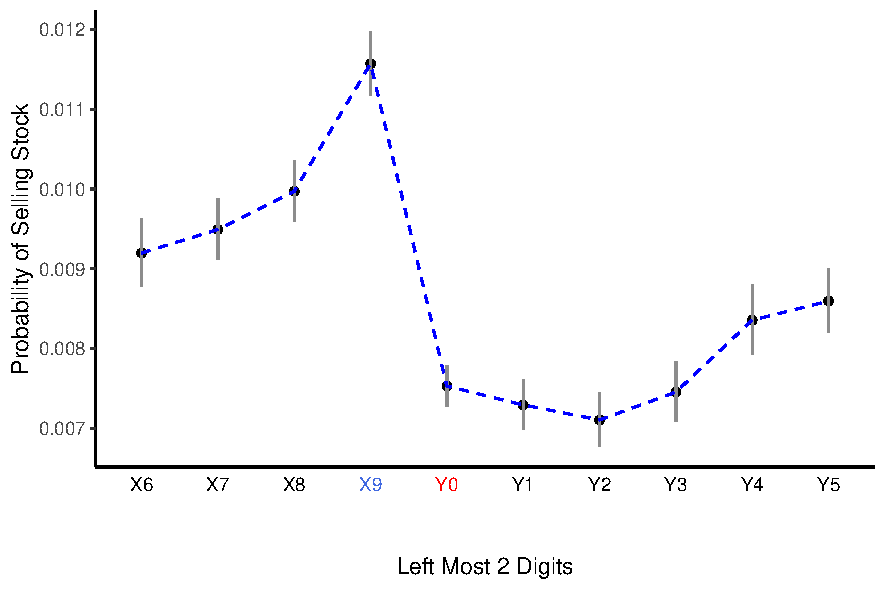
\includegraphics[width=0.45\textwidth]{figures/Left2decrease_probCI_quarter.pdf}
		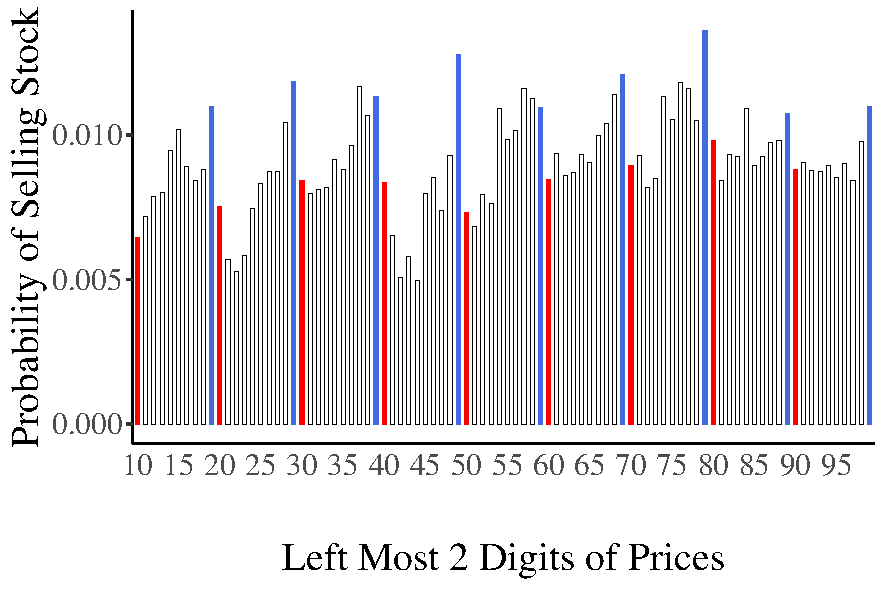
\includegraphics[width=0.45\textwidth]{figures/2left_decrease_quarter.pdf}	
	}
	\fignote{£$Y$ in the X-axes is equivalent to £$X+1$ (e.g., £X9 could include £0.19, £1.9, £19, etc., while £Y0 could include £0.20, £2.0, £20, etc.).}
\end{figure}


\clearpage

\begin{figure}[hbt!]
	\caption{Leftmost Stock Price Digit and Probability of Sale \\ Prices Increasing Sample by Price Range}%
	\label{fig:left_digit_sell_increase_main}%
	\centering%	
	\bigskip
	\subfigure[Price = \pounds0.11 to \pounds1.01]{
		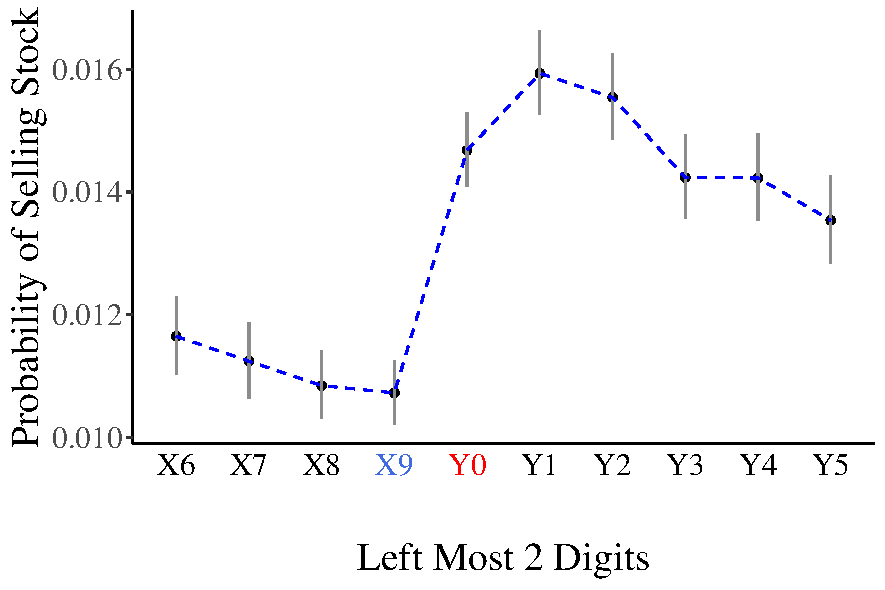
\includegraphics[width=0.45\textwidth]{figures/Left2increases_1pbin_CI_quarter.pdf}
		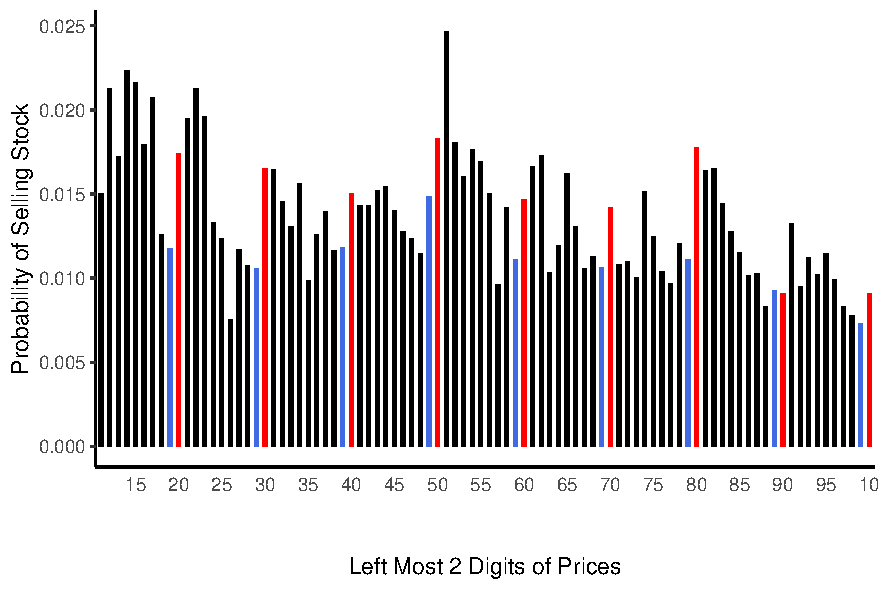
\includegraphics[width=0.45\textwidth]{figures/2left_increase_bin1p_quarter.pdf}
	}
	\subfigure[Price = \pounds1.01 to \pounds10.1]{
		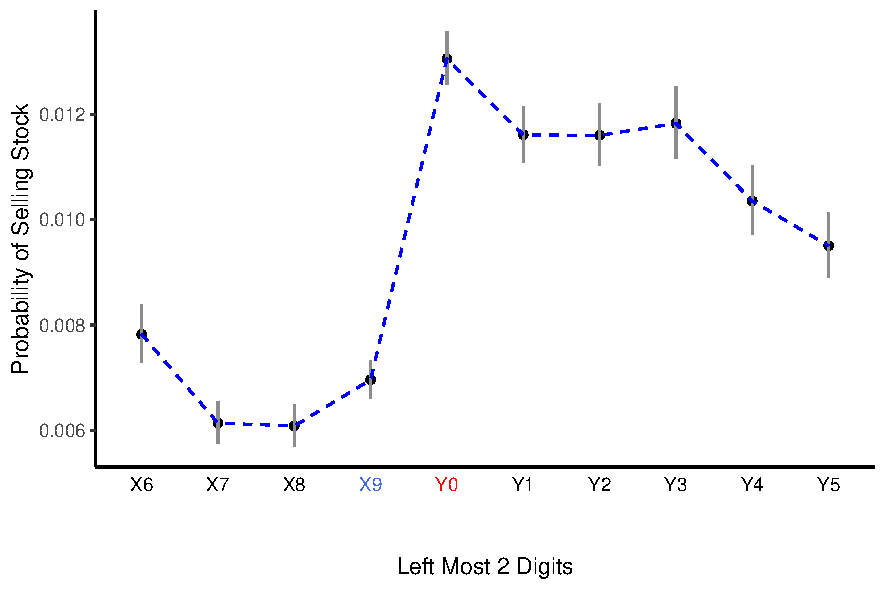
\includegraphics[width=0.45\textwidth]{figures/Left2increases_10pbin_CI_quarter.pdf}
		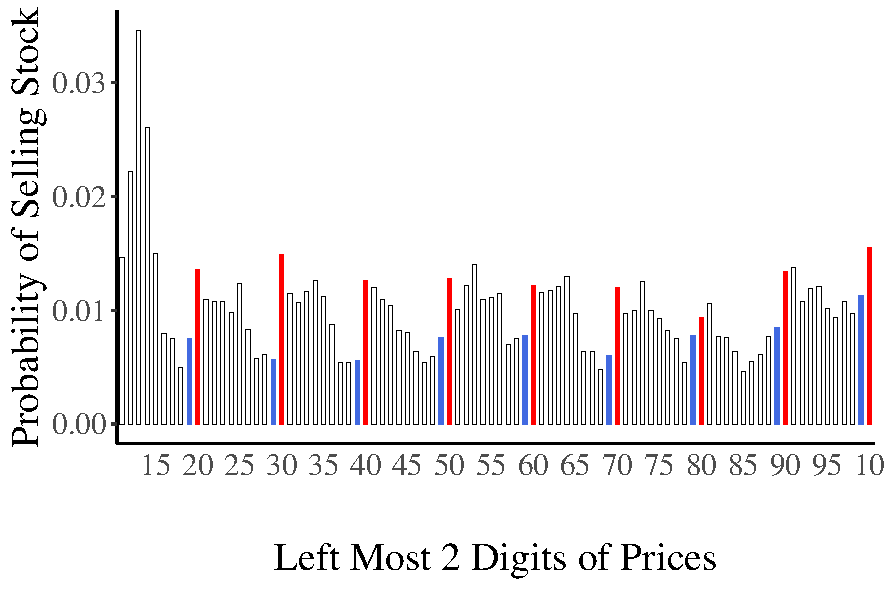
\includegraphics[width=0.45\textwidth]{figures/2left_increase_bin10p_quarter.pdf}
	}
	\subfigure[Price = \pounds11 to \pounds101]{
		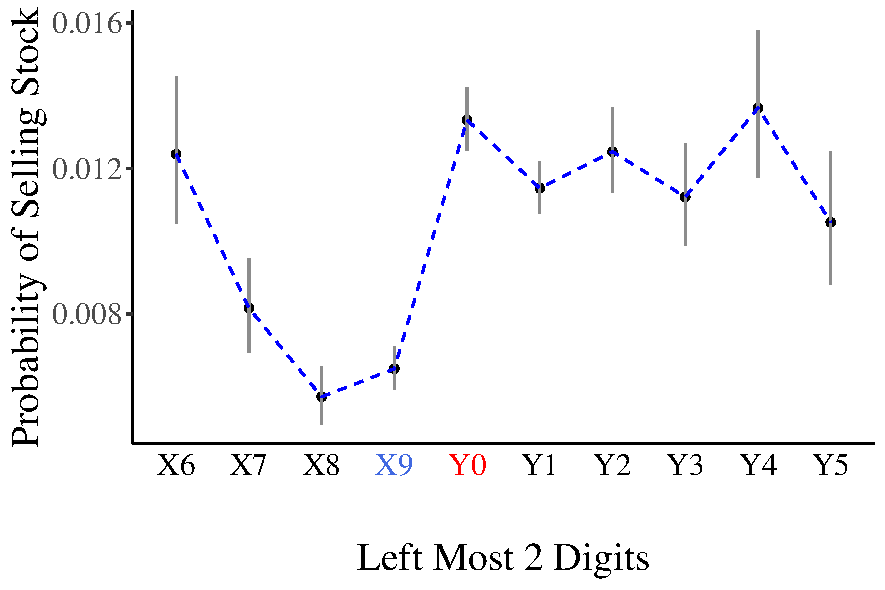
\includegraphics[width=0.45\textwidth]{figures/Left2increases_1poundbin_CI_quarter.pdf}
		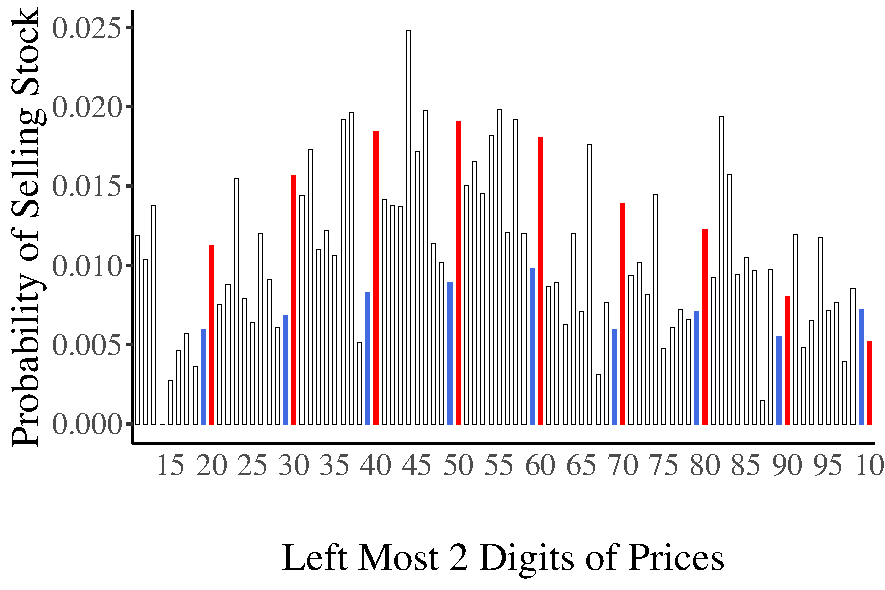
\includegraphics[width=0.45\textwidth]{figures/2left_increase_bin1pound_quarter.pdf}
	}
	\fignote{£$Y$ in the X-axes is equivalent to £$X+1$ (e.g., £X9 could include £0.19, £1.9, £19, etc., while £Y0 could include £0.20, £2.0, £20, etc.). Panels A, B and C show equal size bins of 1p, 10p and £1, respectively. Panel A corresponds to 25\% of the observations in the prices increasing sample; Panel B, to 55\%; and Panel C, to 8\%.}
\end{figure}

\clearpage
\begin{figure}[hbt!]
	\caption{Leftmost Stock Price Digit and Probability of Sale \\ Prices Decreasing Sample by Price Range}%
	\label{fig:left_digit_sell_decrease_main}%
	\centering%	
	\bigskip
	\subfigure[Price = \pounds0.10 to \pounds1.00]{
		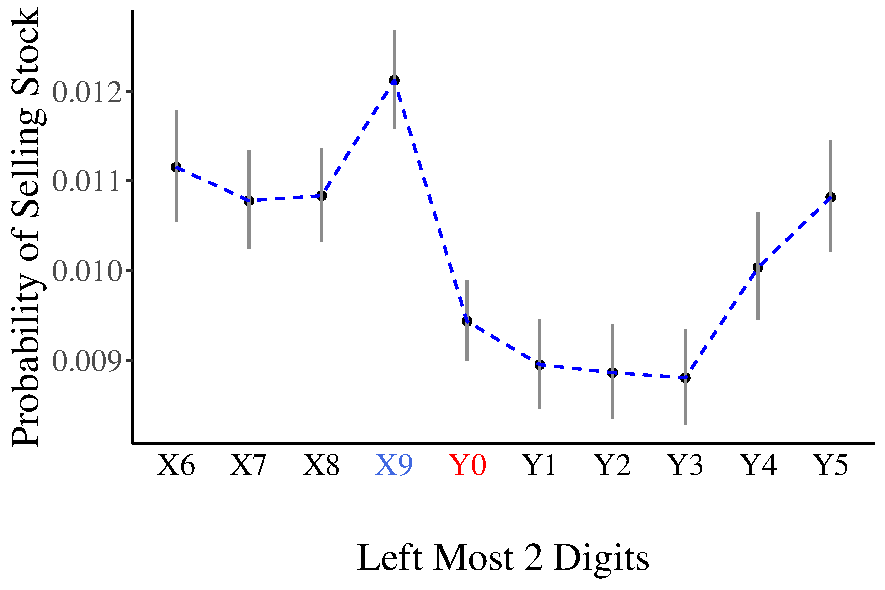
\includegraphics[width=0.45\textwidth]{figures/Left2decreases_1pbin_CI_quarter.pdf}
		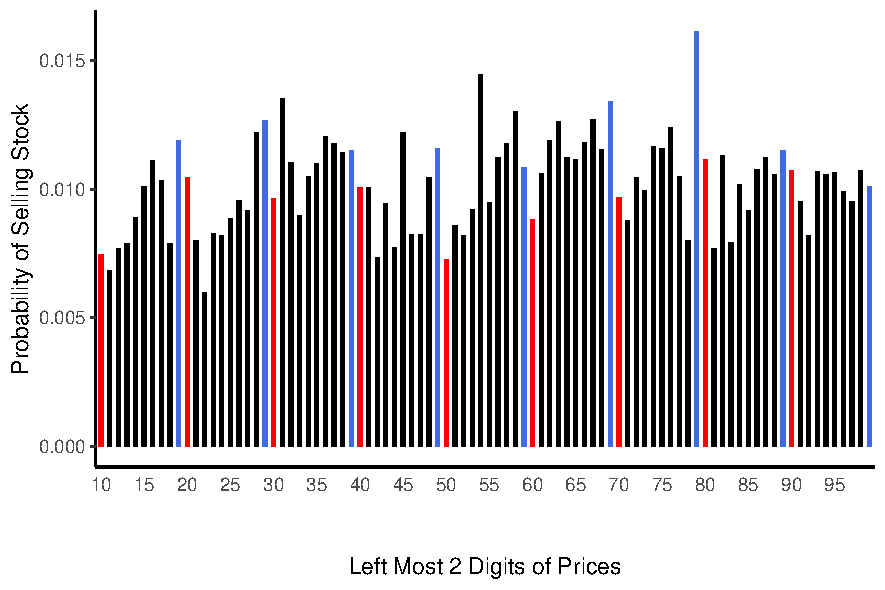
\includegraphics[width=0.45\textwidth]{figures/2left_decrease_bin1p_quarter.pdf}
	}
	\subfigure[Price = \pounds1.00 to \pounds10.0]{
		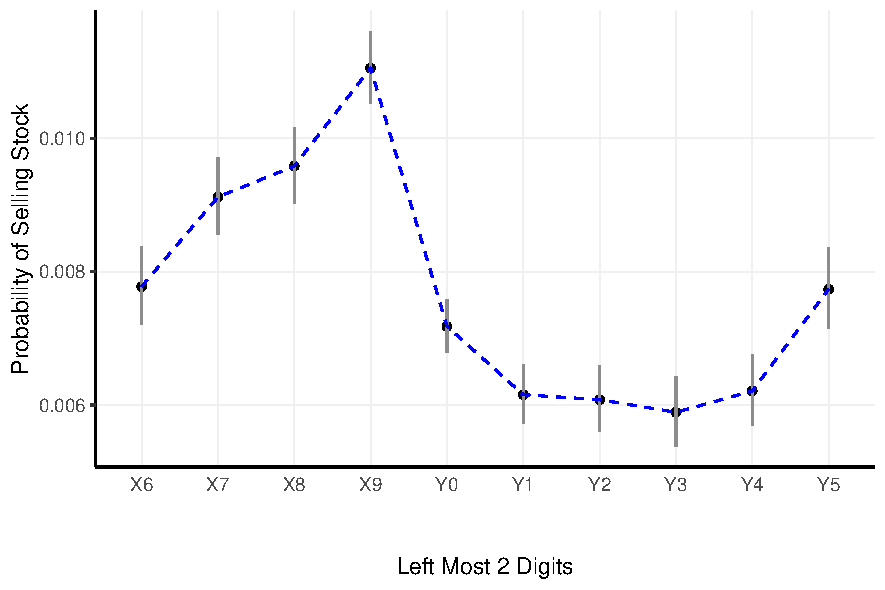
\includegraphics[width=0.45\textwidth]{figures/Left2decreases_10pbin_CI_quarter.pdf}
		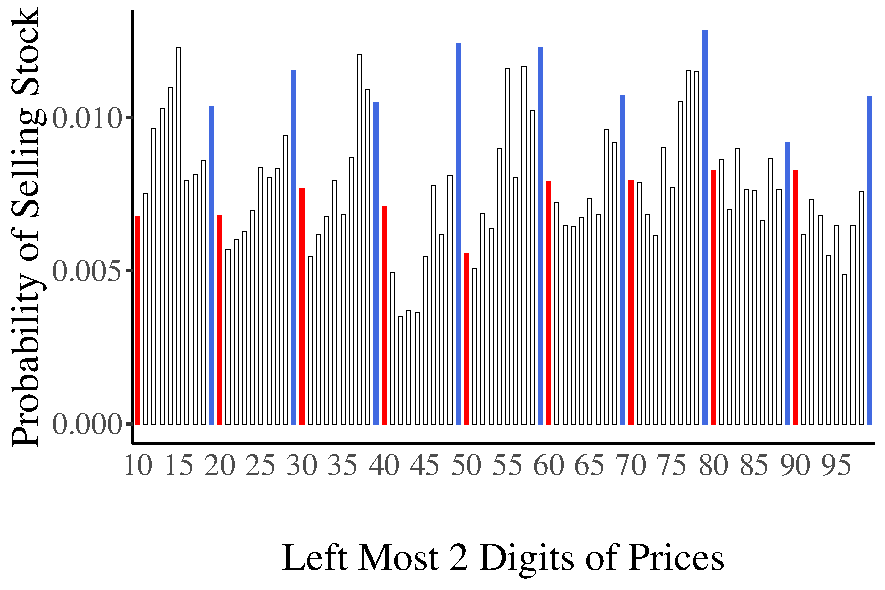
\includegraphics[width=0.45\textwidth]{figures/2left_decrease_bin10p_quarter.pdf}
	}
	\subfigure[Price = \pounds10 to \pounds100]{
		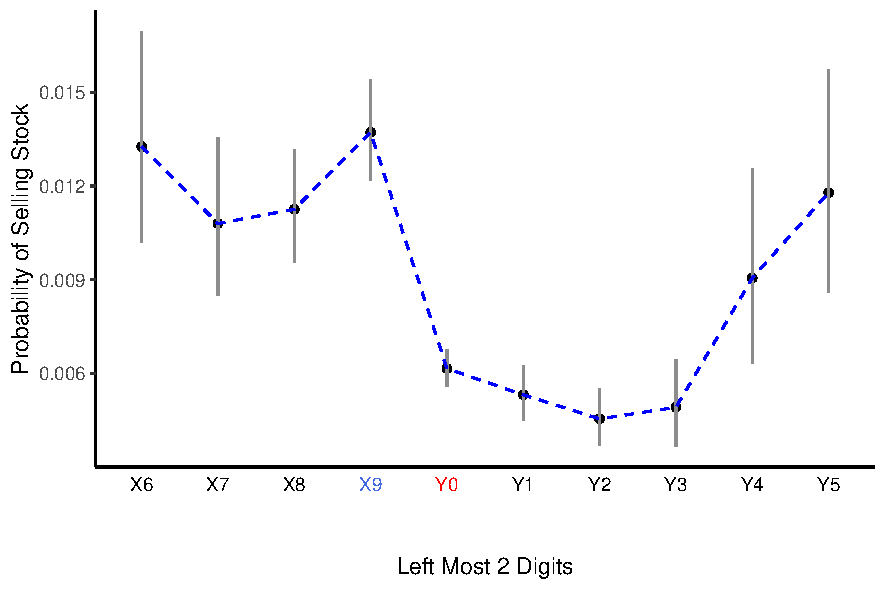
\includegraphics[width=0.45\textwidth]{figures/Left2decreases_1poundbin_CI_quarter.pdf}
		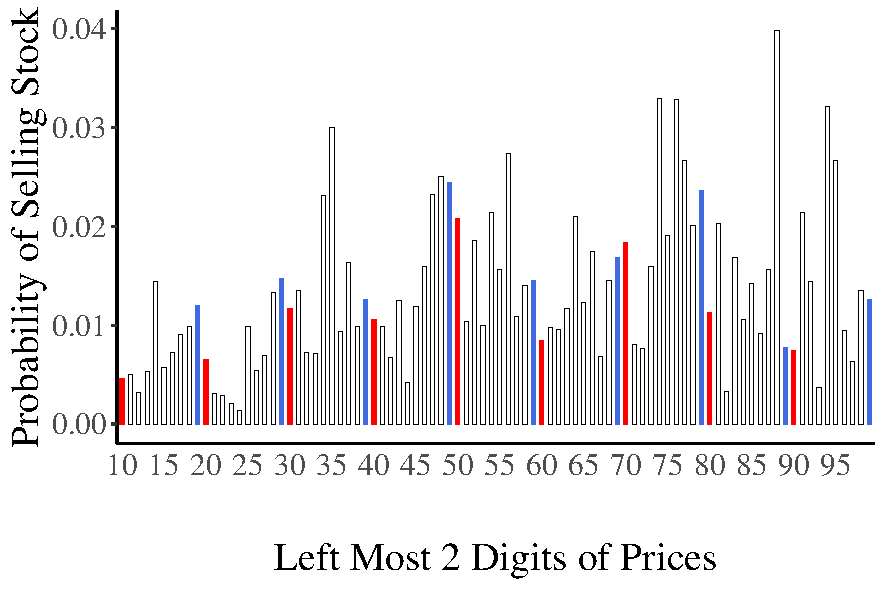
\includegraphics[width=0.45\textwidth]{figures/2left_decrease_bin1pound_quarter.pdf}
	}
	\fignote{£$Y$ in the X-axes is equivalent to £$X+1$ (e.g., £X9 could include £0.19, £1.9, £19, etc., while £Y0 could include £0.20, £2.0, £20, etc.). Panels A, B and C show equal size bins of 1p, 10p and £1, respectively. Panel A corresponds to 27\% of the observations in the prices decreasing sample; Panel B, to 43\%; and Panel C, to 7\%.}
\end{figure}